\documentclass[a4paper,11pt]{article}

\usepackage{graphicx}
\usepackage[sort&compress]{natbib}
\usepackage{pdfpages}
\usepackage{amsmath}
\usepackage{breqn}
\usepackage{amssymb}
\usepackage{float}
\usepackage{listings}
\usepackage[a4paper]{geometry}
\usepackage{hhline}
\usepackage{makecell}

\begin{document}

\title{Using Linear and Flexible Classifiers to Detect Fake Hotel Reviews}
\date{\today}
\author{Jaspreet Singh, 3754022         	\and
        Dani\"el Stekelenburg, 4153286		
}
 
\maketitle

\abstract{Ever wanted to buy something online and read opinions about others who bought the product? Or searched for a nice apartment in a city where you would like to spend your holiday, and looked up the reviews about previous visitors? Well... you need to know that a portion of these reviews are fake! Because these fake reviews can mislead the interested reader, we wanted to know if we can find a way to detect whether a review is fake or not. This paper presents four different classification algorithms and describes their results when learned on a dataset of honest and fake reviews. Their goal is to classify whether a review is fake or honest as good as possible. The results show that the least complex model performs the best, which is an interesting result.}

\section{Introduction}
Nowadays, many companies which offer a product or service, also give the customer the option to post an online review about their experiences with the product itself or the service provided by the company. You may assume that a lot of these reviews are written truthfully, but there seems to be quite a number of reviews which are actually fake. Why would someone do such a thing? Reasons for someone to place a fake review are because that company is a market contender. It is also possible that you are an employee of this company and would like to `improve' its reputation by posting lots of very positive fake opinions on the company's website. %checked

Since fake reviews give false information, consumers might be misled in this case. To prevent this problem, we want to know if it is possible to automatically detect whether a review is fake or not. The goal of this paper is to find a way to determine if a given review is written truthfully or not. If this is the case, companies can use such an algorithm in order to filter out fake reviews, which will help them to maintain an honest review system. %checked

The dataset in this case consists out of hotel reviews that have been collected by Ott et al. \cite{Ott:2011}. This dataset is split into a train set and test set. The train set is used to train the classifiers and the test set is used to estimate the performance of the trained classifiers. %checked

One can look at many aspects of a review in order to detect fake reviews. In this paper we limit ourselves to only the contents of the reviews. This means that other aspects such as the amount of reviews the user has posted, time active on the platform and personal information are not taken into account. For every review some pre-processing is performed to eventually get a document-term matrix. This matrix is then used to train the four individual classifiers that will be used for detection. Two types of classifiers will be tested: linear classifiers and flexible classifiers. The linear classifiers that will be tested are Naive Bayes and Regularized Logistic Regression. The flexible classifiers use classification trees and random forests. Besides describing the behavior of each algorithm when we change certain parameters, the difference in performance between using unigrams or also bigrams will be discussed. %checked

First we will look at the dataset of hotel reviews. Then the methodology will be explained to perform the experiments and evaluate the four classification methods with both unigrams and bigrams. The results of the experiments are then presented, using the data set and the methodology. At last the results are discussed in which we will discuss the performance of four classification methods, whether there is a difference in performance between using unigrams and bigrams, and what terms or couples of words give an indication for honest and fake reviews. %checked

\section{Data}
\label{section:data}
In this section we will take a look at the dataset\footnote{http://myleott.com/op_spam/} we used. We will first discuss the structures of the dataset and how it will be used, then we perform some exploratory analysis on the data. %checked

The dataset used in the experiments consists out of hotel reviews \cite{Ott:2011}. Both fake and truthful reviews are present in the data. This dataset consists out of 1600 reviews in total but since we are only interested in distinguishing between fake and truthful negative reviews, the total number drops down to 800. The dataset is split into a training set and a test set. The training set is used to train the classifiers and consists out of 80\% of the reviews. The test set is then used to estimate the performance of the classifiers, which is the other 20\% of the reviews. Thus, in total we have 640 (4 folds) reviews for training and 160 (1 fold) for evaluation. %checked

The only information from the data set that will be used, are the terms present in the review. The reviews will be pre-processed and transformed into a document-term matrix. The pre-processing is explained in the next section. This matrix indicates for each review (document) which terms are present. The set of terms are all terms used in all reviews. This number can get rather large because everyone used different words and has a different style of writing. To keep the size manageable, pre-processing is required. This means that information on term sequences is lost. We are curious whether including bigrams will reduce this problem. %checked

\subsection{Exploratory analysis} %TODO CHECK, en consistent maken met de rest van het verhaal
Here we look at some general statistics of the provided dataset. The dataset is already pre-processed as described in the methodology section. The document-term matrix contains a total of 776 terms. In Figure \ref{figure:exploratory} the barplots are shown of the top-10 occurring terms in both honest and fake reviews. The top-3 terms for both honest and fake reviews are exactly the same, the relative frequencies also seem to be the same. It will be impossible to distinguish between honest and fake reviews using the top-3. The differences start from the 4th term onwards, here the relative frequencies start to change as well the terms. The term `night' does not appear in the top-10 of honest reviews, this might be an indication that the usage of the term `night' indicates a fake review. In total 6 terms occur in both, 4 out these 6 occur in the exactly the same rank. This means that some terms are not very useful when is comes down to labeling 
\begin{figure}[H]
\label{figure:exploratory}
  \centering
      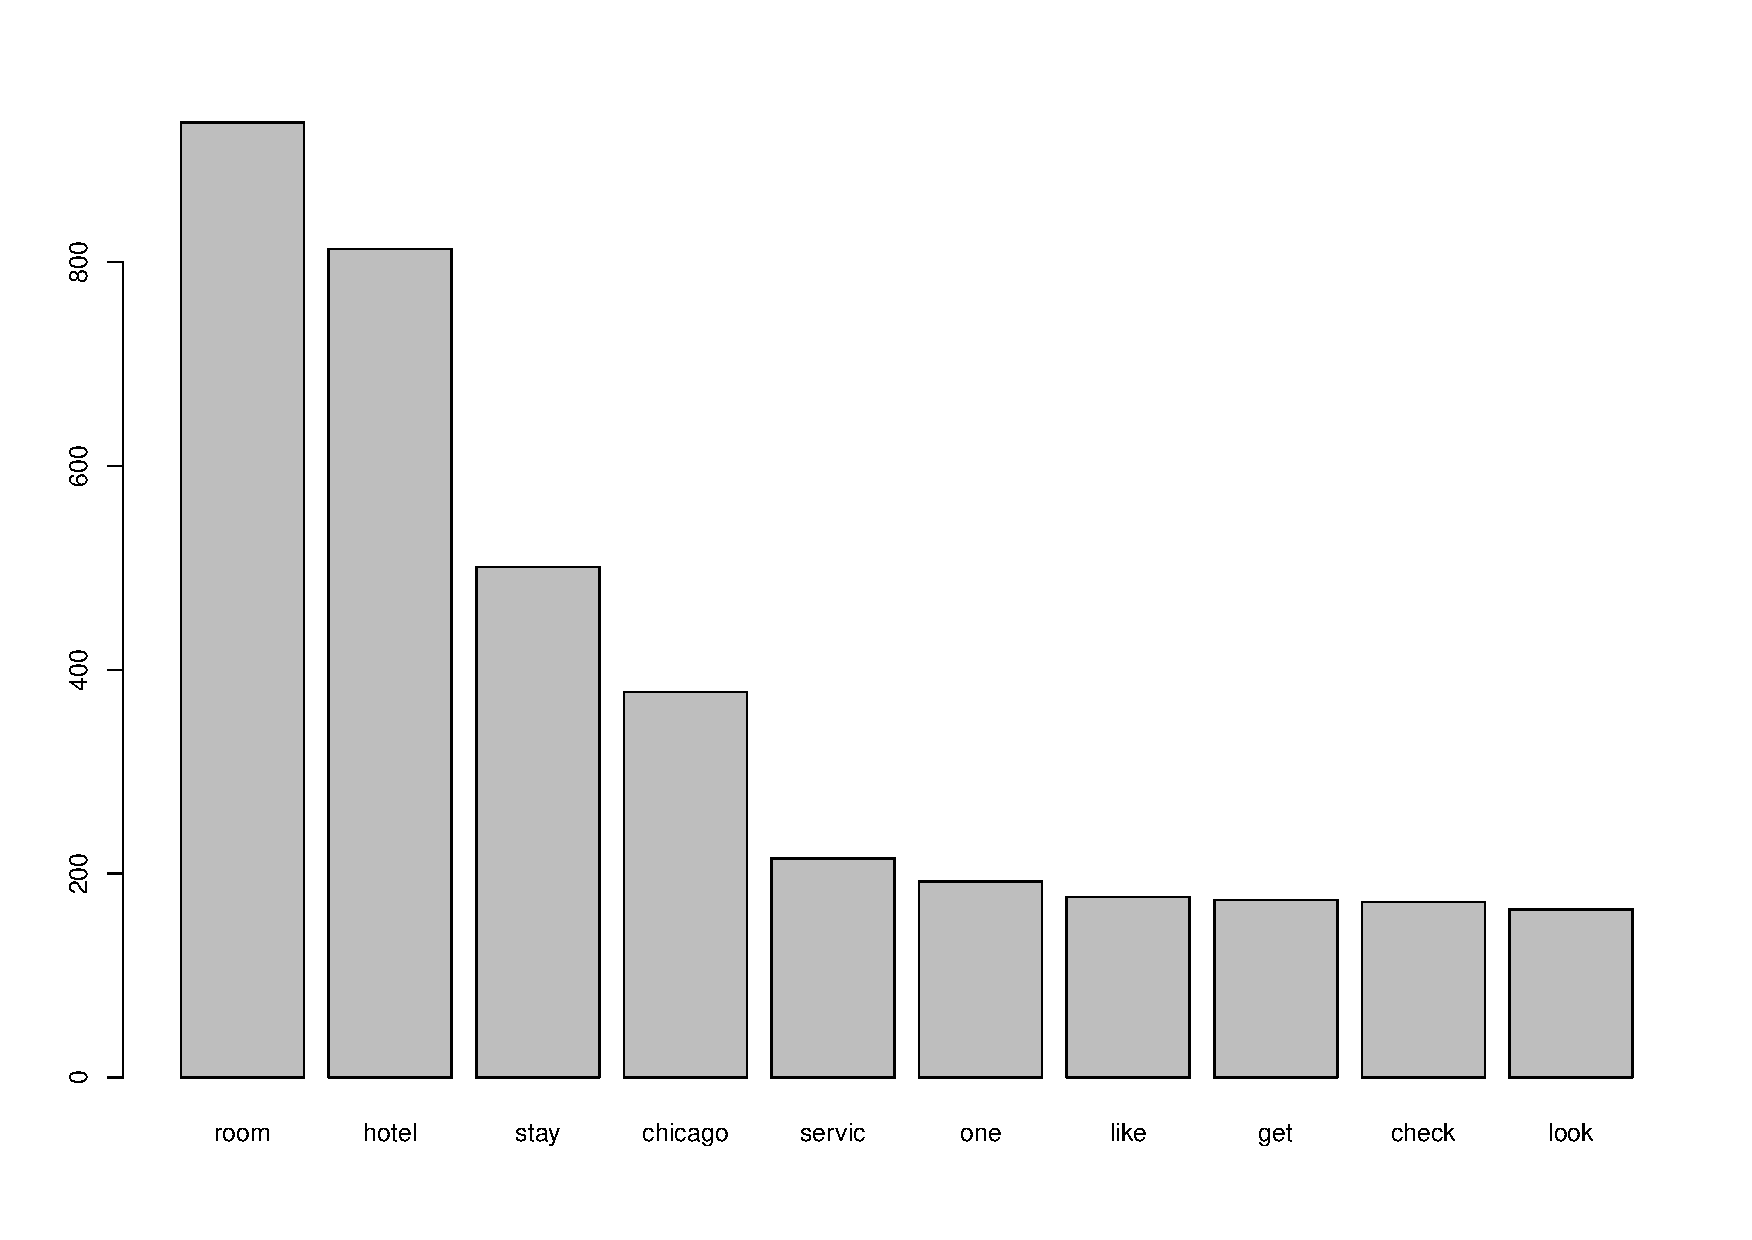
\includegraphics[width=0.65\textwidth]{honest}
      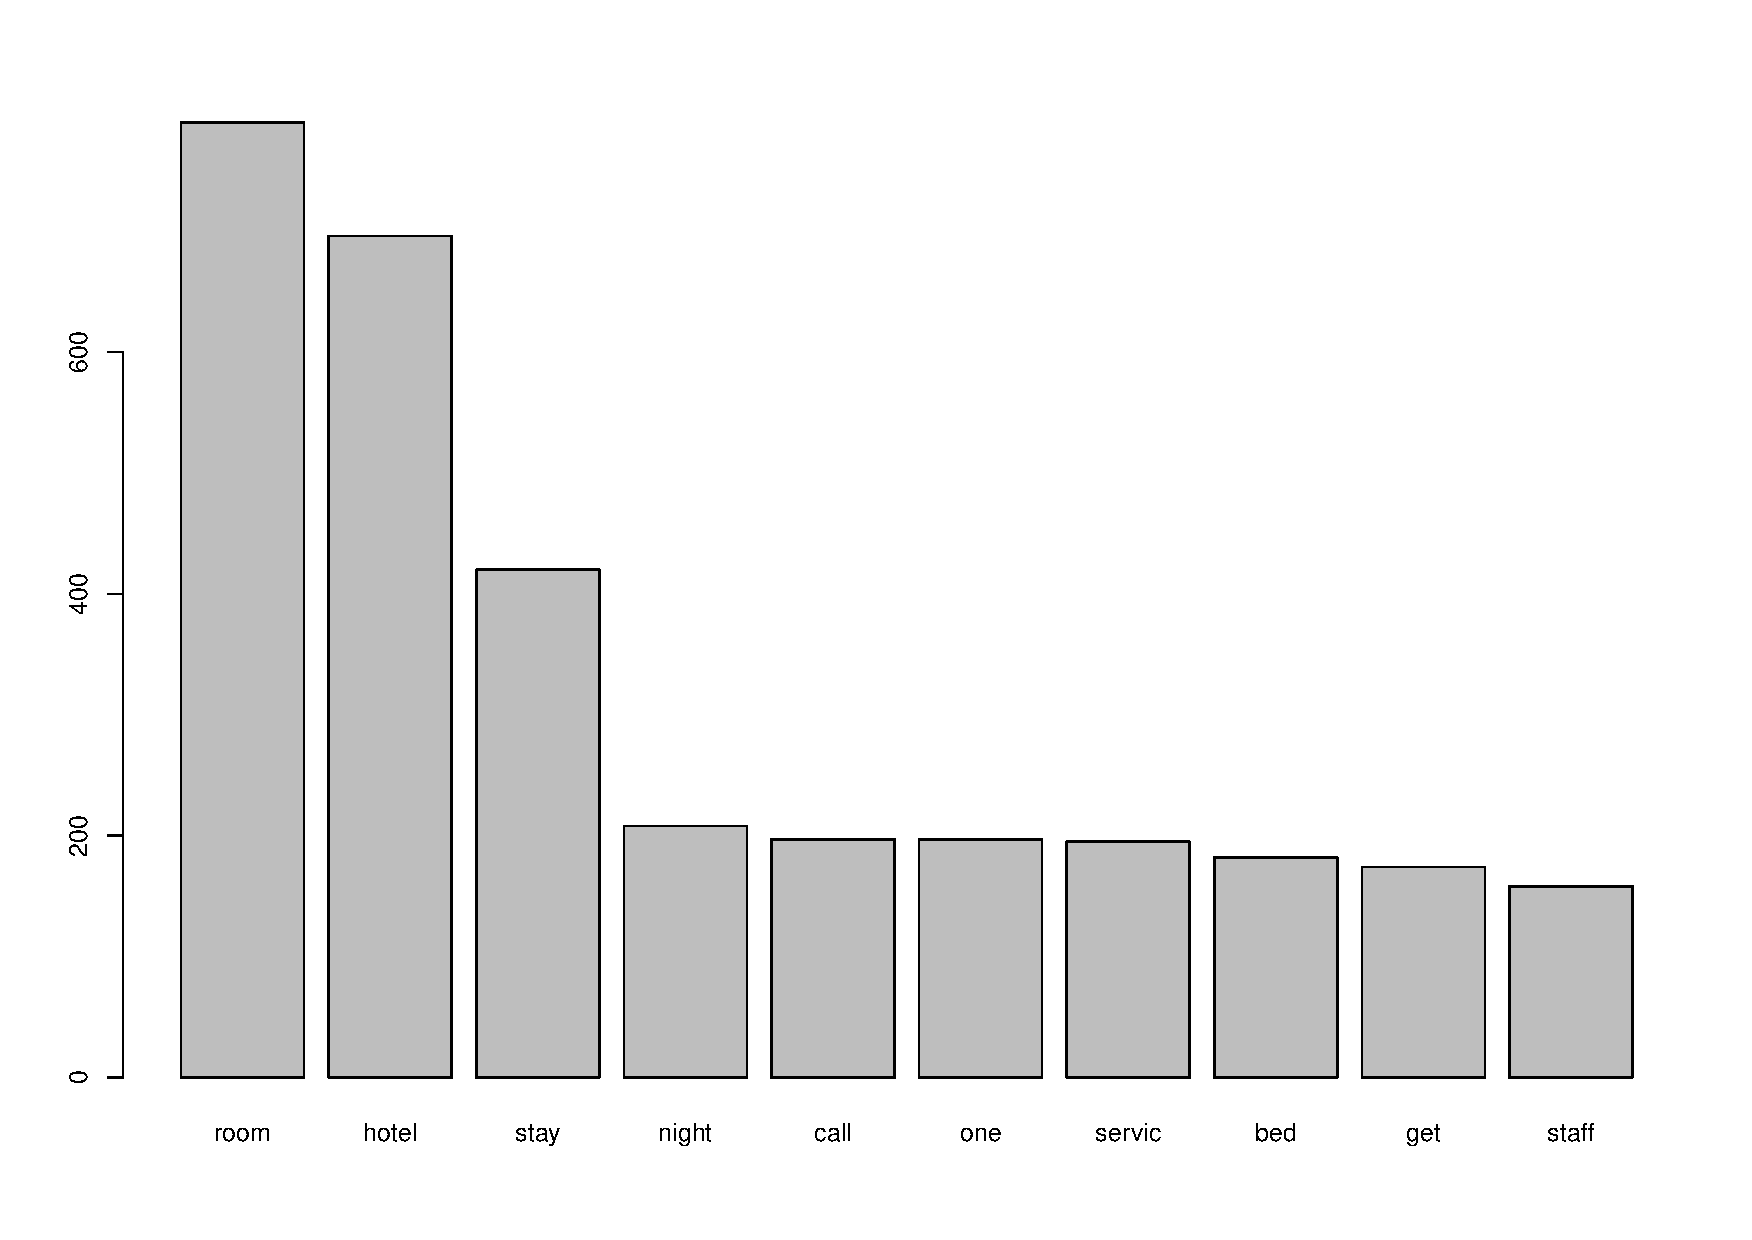
\includegraphics[width=0.65\textwidth]{fake}
  \caption{Top: The barplot of the top-10 occurring terms in honest reviews in terms of frequency. Bottom: The barplot of the top-10 occurring terms in fake reviews in terms of frequency.}
\end{figure}

\section{Methodology}
In this section, the methodology to perform the experiments is argued. This way the reader can reproduce and verify the results that are presented later on. %checked
The whole process of our experiments bassically consist of the following steps:
\begin{enumerate}
\item Pre-processing phase: Make the data set ready to be used, but also apply feature selection (removing/adding features which can reduce/improve the eventual performance of the classifier you want to create).
\item Building a classifier: which is trained on the defined train set, and tested on a test set.
\end{enumerate}

How we implemented these steps will be discussed in detail in this section.

\subsection{Pre-processing functions}
\label{section:pre_processing}
Pre-processing is a not only a way to make the raw data set ready for your classification algorithm. Feature selection is also a part of this phase. Feature selection makes your complete collection of data smaller by filtering out irrelevant pieces of information. More specifically, we wanted to decrease to total size of the document-term matrix of the train set because this will improve the runtime of computing a classifier. Also, a smaller matrix means that you need less memory for storing.%checked

In our case, pre-processing is basically done by adjusting the text within the documents - before the doc-term matrix is created - and by removing certain features from the matrix afterwards. Of course, it is important that applying pre-processing functions does not worsen the eventual classification too much. The perfect scenario is that pre-processing improves your classification. Let's see how the pre-processing steps we applied, and explained in more detail earlier in the paper, influence the document-term matrix.%checked

Here we will look at the steps required to make the dataset ready for training and testing. Since we are only looking at the occurrences of terms in reviews, the order of terms is neglected mostly (not for bigrams). This means that punctuation does not matter anymore, so this can be removed at first. Since we are comparing terms (strings), the capitalization of letters should not matter because `Great' is the same as `great' for example, for this reason all terms are transformed to be in lower case only. %checked

The term \textit{stop words} refers to those words which are most common in a language. Stop words are removed as terms because they appear very frequently in both fake and honest reviews. Therefore, they add little value when it comes down to the classification of a review containing such a word. %checked

In some reviews there might be some extra whitespace between or after terms. Since whitespace itself is not a term, the excess whitespace is removed. Also numbers without context do not give very much information. These terms are removed as well. Applying all these transformation results in a smaller document-term matrix. Without these transformations the matrix will be very large (high dimension) and sparse, and will cause the performance of some classifiers to be very bad.%checked

The removal of sparse terms is another important pre-processing step which we used. Lots of words are being used very few times. However, when you set up a term-document matrix, you include literally every word which occurred in the given data set. This matrix becomes very big quickly, which leads to more time needed for computations. In order to decrease the size of this matrix, we decided to remove all terms which occurred in less than 2\% of the reviews. These terms are what we call the \textit{sparse terms}. Since they rarely occur in the dataset, the impact of these terms in the eventual classification becomes very small. In short, removing these terms is a decent way to decrease the number of features, while keeping the most important features.%checked

There are also other methods we did consider for pre-processing of the data, but did not use eventually. One of these things is the removal of diacritics to normalize the terms. The use of diacritics has become very uncommon in the English language. The only place where they still occur are in names and loanwords from other languages, this is the reason why these have not been removed. %checked

We also did consider the presence of typo's in the reviews. The software package used did not support dealing with typo's. The presence of typo's is greatly removed when removing sparse terms but being corrected would have been the better solution, because they might contribute to the non-sparse terms. We also made no distinction between abbreviations and terms.
The application of stemming is also a step which we eventually did not include in the pre-processing phase. Stemming seems to affect the performance resulting classification a lot. It seems that a lot of information about the label of a review lies in inflected or derived words. Reducing these words to their root form - or \textit{word stem}, leads in our case to classifiers with worse performance than those when stemming is not applied. %checked

Abbreviations can be mapped to their actual meaning. The software package did not support this. Now the abbreviations will be reduced to terms with no dots between the characters. Synonymy and polysemy are two problems that we did not deal with. Synonymy is the case in which two different words have the same meaning (car and automobile). We cannot deal with because a document-term matrix cannot capture these relationships. Polysemy is the case in which a single term has multiple meanings. In this case we do not use any contextual information so the different meanings of polysemy terms cannot be detected. For both unigrams and bigrams, the same steps are performed in the same order. First all the steps are performed except removing the sparse terms, then the bigrams are created because we have not created a document-term matrix yet, then we create the bigrams and remove the sparse bigrams. After this we create the document-term matrix. A bigram feature is considered to be sparse when it occurs in less than 2\% of the reviews. This value is lower than the value of the unigram features, because the total occurrence of bigrams is generally lower than the occurrence of just unigrams. %checked

\subsection{Classifiers}
The four used classification methods for the experiments are Naive Bayes, Regularized Logistic Regression, Classification Trees and Random Forests. For each of the methods its workings are briefly explained and also the some benefits and drawbacks are discussed.

\subsubsection{Naive Bayes Classifier}
A Naive Bayes classifier is a probabilistic classifier, this means that it assigns a probability to each class. Naive Bayes is called a generative model. In classification we are interested in the probability $P(c|d)$. Generative models use Bayes' rule to estimate to estimate this probability. The classes in this case are the \textit{honest} and \textit{fake} reviews. It assigns to the class with highest probability given a review. In the document-term matrix each document is presented by a set of terms, which is also called a set of features. To be more formal, the predicted class class $\hat{c} \in C$, where $C = \{\texttt{fake},\texttt{honest}\}$, given a document $d$ is: \[\hat{c} = \arg\max\limits_{c \in C} P(c|d) = \arg\max\limits_{c \in C} P(x_1, \ldots,x_m|c)P(c)\]
In Naive Bayes the assumption is made that the features are independent within each class, in this case the assumption is that all terms occur independent of each other within each type of review. So the class predicted by Naive Bayes is:
\[
c_{\texttt{NB}} = \arg\max\limits_{c \in C}\log P(c) + \sum\limits_{i=1}^{m}\log P(x_i|c)
\]
Naive Bayes makes two kinds of independence assumptions. The first assumption is conditional independence, which means that all terms occur independent of each other. The second assumption is positional independence. This means that the probability of a term occurring, given the class is independent of the position or order of the terms. These independence assumption do not hold for the reviews, or any document written in a natural language. This means that the independence assumptions are badly violated, so the calculated probabilities will be way off. The goal of classification is not to accurately estimate probabilities but to predict the correct class. As long as the relative probabilities are correct in most cases, classification performance will not be hurt by it. Another benefit of Naive Bayes is that it requires estimation of relatively few parameters, furthermore it is also fast and has low storage requirements.  

When training the model, first the class priors are estimated as the proportion of number of documents for class $c$ with respect to the total number of documents in the training set $\hat{P}(c) = \frac{N_c}{N_{doc}}$. The word probabilities are then estimated as: \[\hat{P}(x_i|c) = \frac{count(x_i, c)}{\sum_{x_j\in T} count(x_j, c)}\] This is the number of occurrences per term in the class proportional to the number of occurrences to all terms, where $T$ is the set of all terms in the document-term matrix.

In Naive Bayes the features are the terms in the document-term matrix. The features used here are those which are the result of the pre-processing described before. 

\subsubsection{Regularized Logistic Regression}
\label{section:logitRegressionExplained}
In contrast to generative models, there also exist discriminative models which model $P(c|d)$ directly. These models only model the conditional distribution of the class given a document. The probability of $d$ is not modeled. For binary classification problems we use $P(c|d) = f(d,\beta)$, where $f(d,\beta)$ is some deterministic function of $d$. A document in this is case a vector containing the terms that appear in it, and $\beta$ is a vector containing weights for each of the terms. The logistic response function then is: $P(c|d) = (1+e^{-\beta^Td})^{-1}$. The odds of a review being fake can be formulated as $P(c = \texttt{fake} | d) / P(c = \texttt{honest} | d)$. We want the review as being fake if $P(c = \texttt{fake} | d) > P(c = \texttt{honest} | d)$, this is the case when $P(c = \texttt{fake} | d) / P(c = \texttt{honest} | d) > 1$, or $\ln (P(c = \texttt{fake} | d) / P(c = \texttt{honest} | d)) = \beta^Td > 0$. 

The weights in $\beta$ are estimated by using maximum likelihood (ML) estimation. Here we assume that all reviews have been written independent of each other. So the probability that a review is fake $(c = 1)$ or honest $(c=0)$ is $P(c) = p^c(1-p)^{1-c}$, generalizing over $n$ independent reviews we get \[P(c1,\ldots,c_n) = \prod\limits_{i=1}^{n}p^{c_i}(1-p)^{1-c_i}\], which is the likelihood function for observing the sequence of $n$ with their respective classes. The log likelihood then is: 
\[\ln P(c1,\ldots,c_n) = \sum\limits_{i=1}^{n}\ln p^{c_i}+\ln (1-p)^{1-c_i}\] The maximum is computed by taking the derivative and equating it to zero. We still have not incorporated the document contents into the obtained probability distribution. The probability $p_i$ of classifying a document $d_i$ as being fake is now defined as $p_i = (1+e^{-\beta^T d_i})^{-1}$, and the probability $1-p_i$ of classifying a document $d_i$ as being honest is then $1-p = (1+e^{\beta^T d_i})^{-1}$. Since the observations are independent for $c_i$, we get the following log-likelihood function: 
\[l(\beta) = \ln P(c|\beta) = \sum\limits_{i=1}^n \{c_i \ln p_i + (1-c_i)\ln(1-p_i)\}\]
We want to maximize the function, so we have take the derivative of $l(\beta)$: $g(\beta_j) = \sum\limits_{i=0}^n (c_i-p_i)d_{ij}$, we now have to solve $g(\beta_j) = 0$. The optimal solution obtained is $\sum\limits_{i=0}^n c_i d_{ij} = \sum\limits_{i=0}^n p_i d_{ij}$.

When we have a large number of terms, this method might result in overfitting the model. This can be controlled by `punishing' large weights in either spectrum. A penalty term is introduced based on the number of coefficients, this is called to the LASSO penalty: \[E(\beta) = -l(\beta) + \lambda\sum\limits_{j=1}^{m} |\beta_j|\] This is the error that we want to minimize, where the value of $\lambda$ is selected using cross-validation. We take the the least complex value of $\lambda$ such that it is at most 1-standard error away from the minimum to prevent overfitting.

\subsubsection{Classification Trees}
\label{section:classTreesExplained}
Where Naive Bayes and Regularized Logistic Regression are considered as linear models, classification trees are considered to be flexible models. A classification tree works by following a path, where every node represents a feature, until a leaf node is reached. In a leaf node the class of the review is determined. The path chosen depends on a condition for the considered feature in every non-leaf node. Every node stores the records from the training set that are considered, with for every possible class the number of documents that belong to each of the classes. Every edge from one node to the other contains a condition, which is based a value of the feature of the upper node. In this case every node will hold a term, and the split is based on whether a review contains the term or it does not contain the term. In the leaf nodes the class assigned is the majority class. 

Building a classification is done by using the notion of impurity of a node. The more `pure' a node is, the better the ability is to distinguish between classes. The ideal situation is where a node only contains observations that belong to a single class. A measure which indicates the distance to this ideal is called an impurity measure. The impurity $i(t)$ of a node $t$ is denoted as a function of the relative frequencies of the classes in $t$: $i(t) = \phi(p1,\ldots,p_J)$, where $p_j(j=1,\ldots, J)$ are the relative frequencies of the $J$ different classes in node $t$. In our case we only have two classes, so that makes life more easy. The more impurity we can reduce, the better split we can obtain. The quality of a binary split $s$ in node $t$ is defined as the reduction of impurity $\Delta i(s,t) = i(t) - \{\pi(l)i(l)+\pi(r)i(r)\}$, where $l$ is the left child of node $t$, $r$ is the right child of node $t$ and $\pi(l)$,$\pi(r)$ the proportion of cases that were sent to the left and right respectively. There are many impurity functions available, the one that will be used for the experiments is called the Gini-index. For the binary case the Gini-index is: $i(t) = p(0|t)p(1|t) - p(0|t)p(1-p(0|t))$, where 0 and 1 represent a review as being honest and fake respectively, and $p(c|t)$ is the relative frequency of class $c$ in node $t$. 

The tree is constructed by iteratively choosing the nodes with the highest impurity reduction until there are no nodes left to consider. The problem with this `naive' approach is that it is very prone to overfitting. Stopping rules limit the size of the tree by setting a threshold on the impurity reduction to not further expand a node. A disadvantage of this method is that sometimes a weak split is required to be followed by a good split. The problem can be avoided by using pruning. Here we first grow a very large tree and then prune this tree. The objective is to select the pruned subtree which has the lowest true error rate. The method we used is cost-complexity pruning. Here want to find a balance between fit and complexity. The total cost $C_\alpha(T)$ of tree $T$ is: $C_\alpha(T) = R(T) + \alpha|\tilde{T}|$, where $R(T)$ is the ratio of number of wrong classification made by $T$ and the number of examples in the training sample which is also called the resubstitution error, and $\alpha|\tilde{T}|$ is a penalty for the complexity of tree $T$. Based on the values we use for $\alpha$, the best tree which has the lowest error rate on the test set $R^{ts}(T)$, this en estimation of the true error rate. The selected final tree is the smallest tree with $R^{ts}$ within one standard error of the minimum to prevent overfitting. This selection process is performed by using cross-validation. 
 
%parameters\features
\subsubsection{Random Forests}
Single classification trees are generally not among the top predictors. A committee of trees might work better. With random forests, every time we have to determine the best split in a node, we first randomly select a subset of features we will consider for that split. Classification trees are know to have high variance in their predictions. This can reduced by averaging by using bootstrap sampling. This means we draw a sample with replacement from the training set. The total number of samples drawn is equal to the number of reviews we have in the training set. We construct a classification tree on this sample. This is repeated $M$ times to create $M$ different trees. For prediction, each tree in turn makes a prediction, where the majority vote of all predications is taken as the final predication. This averaging in the predication, lowers the variance compared to single classification trees.

%parameters\features
\subsection{Evaluation}
\label{section:evaluation}
To make statements on the performance of the classifiers, the following four measures will be used: accuracy, precision, recall, and F1-score. Accuracy in this case will give information on the ability to correctly classify fake and genuine reviews. The precision indicates the ability to actually detect fake reviews. The recall indicates the ability to classify a review as fake given it is actually fake. The F1-score is the harmonic mean of the precision and recall. Based on the true labels and predicted classes we can construct a confusion matrix as per Table \ref{table:conf_matrix}.
\begin{table}[ht]
\centering
\begin{tabular}{|l||l|l|}
\hline
 \shortstack{actual class $\rightarrow$ \\ predicted class $\downarrow$} & fake   & honest   \\
  \hhline{|=||=|=|}
fake & True Positive (TP) & False Positive (FP) \\
honest & False Negative  (FN) & True Negative (TN) \\
\hline
\end{tabular}
\caption{The representation of each cell in a confusion matrix.}
\label{table:conf_matrix}
\end{table}
The true positives (TP) are the number cases predicated as being fake, that are also actually fake. The true negatives (TN) are the number of cases predicted as being honest, that are also actually honest. These two are the values that represent what has been classified correctly. The false negatives (FN) are the number of cases predicated as being honest but are actually fake (type-II error). The false positives (FP) are the number of cases predicted as being fake but are actually honest (type-I error). These two are the values that represent what has been classified incorrectly.

The values for the accuracy $A$, precision $P$, recall $R$ and F1-score can be easily computed after we have obtained the results for each of the methods.
\[
A = \frac{TP + TN}{TP + TN + FP + FN}
\qquad
P = \frac{TP}{TP+FP}
\qquad
R = \frac{TP}{TP+FN}
\qquad
F_1 = 2\times\frac{P \times R}{P+R}
\]

When we want to compare for two methods, or between unigrams and bigrams for a given method if their performance is significantly different in terms of the accuracy, we first have to determine how many cases are classified correctly by the one and incorrectly by the other, and vice versa. We call these numbers $n(A)$ and $n(B)$. The cases predicted correctly by both are ignored, because we are only interested in the cases where they differ from each other. If both methods have the same accuracy, then P(correct by A and incorrect by B) = P(incorrect by A and correct by B) = 0.5. If either one of the events occurs, we call this a success. We perform a Bernoulli experiment with $n(A)+n(B)$ trials and probability of success of 0.5. This will determine the probability of observing an outcome which is as extreme or more extreme than the observed outcome. This probability is the $p$-value of the test. We say that there is a significant difference in the accuracy when $p<0.05$. The null hypothesis $H_0$ is that both methods perform similarly, with the alternative hypothesis $H_1$ being that they do not perform similarly. This experiment will be conducted to test whether there is a significant difference between the three classification methods.

\section{Results}
This section describes the results of our findings when experimenting with the different algorithms. At first, we will take a look at the influence of the pre-processing steps. Then, the resulting classifiers of Naive Bayes, Regularized Logistic Regression, classification trees and random Forests will be shown. Here, we make a distinction between the classifications of only using unigrams (features which represent just one term in a document) and including bigrams (features representing pairs of consecutive terms in a document, like "never forget").

\subsection{Experimental Setup}
\label{section:expSetup}
We have implemented the four classification methods using the R programming language. For Naive Bayes, we used the \textit{tm} package\footnote{https://cran.r-project.org/web/packages/tm/index.html}. The implementation of Regularized Logistic Regression with LASSO is done with the package \textit{glmnet}\footnote{https://cran.r-project.org/web/packages/glmnet/index.html}. Package \textit{rpart}\footnote{https://cran.r-project.org/web/packages/rpart/index.html} is used for the classification tree method and package \textit{randomForest}\footnote{https://cran.r-project.org/web/packages/randomForest/index.html} is used for the random forest method. At last, we used package \textit{RWeka}\footnote{https://cran.r-project.org/web/packages/RWeka/index.html} to include bigrams as features.

Since regularized logistic regression, classification tree and random forest already have feature selection implemented, these methods do not need much pre-processing beforehand. For these three algorithms, we only apply basic pre-processing steps to clean up the text in the dataset, which do not remove any words. These steps remove punctuation, sets all text to lower and removes excess whitespace.

Unlike the other algorithms, Naive Bayes is strongly dependent on the pre-processing phase. That is why we added a couple of steps in this phase.


\subsection{Unigrams}
Now we will show you the classifiers of the different methods that we have used. These classifiers are based on unigrams. The term \textit{unigrams} already have been explained shortly. It means that the document-term matrix used only contains features which stand for a single word. In the next section, the difference between only using unigrams as features and unigrams + bigrams as features is discussed.

\subsubsection{Naive Bayes Classifier}
The first algorithm we used for classification is the Naive Bayes classifier. Like we already explained in Section \ref{section:expSetup}, pre-processing has a big influence on the performance of this classification method. Because of this, we are interested in the impact of adjusting the steps in the pre-processing phase on the performance and runtime of Naive Bayes. This impact is described below.

Starting off with the original document-term matrix of the training set, the size of this matrix is 640 by 11355 (640 are the number of reviews, 11355 different terms found). In Table \ref{table:pre-processing} you can see the number of features decreases when we apply these pre-processing steps in the given order (first removing punctuation, then setting all text to lower case etc.). Finally, we maintain only 776 features, which leads to a much smaller matrix (640 by 776) than the original one (640 by 11355). 

\begin{table}[H]
\centering
\caption{Number of features after applying each pre-processing step.}
\label{table:pre-processing}
\begin{tabular}{|l|c|}
\hline
                                   & \# of features \\
\hline
Raw size                           & 11355          \\
1. Remove punctuation                 & 7203           \\
2. Text to lower                      & 7203           \\
3. Remove excess whitespace           & 7203           \\
4. Remove numbers           		   & 6994           \\
5. Remove stop words                  & 6897           \\
6. Remove sparse terms (\textless2\%) & 776           	\\
\hline
\end{tabular}
\end{table}

The last step which removes sparse terms, greatly decreases the number of features. We were interested the difference in the accuracy and runtime of a classification where we used this pre-processing step and one where we did not. For this example, we used Naive Bayes. In \ref{table:pre-configs} you can see the corresponding accuracy and runtime for three difference configurations. One where we did not apply any pre-processing, one where we applied every pre-processing step but kept the sparse terms, and one where all pre-processing steps were applied. In Table \ref{table:pre-configs}, the resulting accuracy and runtime are shown.

\begin{table}[H]
\centering
\caption{Naive Bayes applied after different pre-processing configurations.}
\label{table:pre-configs}
\begin{tabular}{|l|l|l|l|}
\hline
Pre-processing set-up 			 & \# of features & Accuracy & Runtime (in sec.) \\
\hline
No pre-processing                & 11355          & 85\%     & 2586.63           \\
All pre-processing steps, except last step & 8907           & 81,88\%  & 419.25            \\
All pre-processing steps         & 776            & 81.88\%  & 9.09              \\
\hline
\end{tabular}
\end{table}

Note that the runtime is almost 50 times bigger when we include the 2\% sparse terms in our document-term matrix, but the accuracy stays the same. This shows that removing sparse terms is a big improvement on the runtime of the algorithm, without lowering the performance. Also recall that we are `only' The runtime of bigger classification queries will become infeasible otherwise and we want our classifications to classify the defined test set within a couple of seconds. 

Thus, we prefer the Naive Bayes classifier over the other variants. The performance of this classifier is included in Table \ref{table:performanceOverview}.

\subsubsection{Regularized Logistic Regression}
Regularized Logistic Regression is the second method which we implemented for classifying reviews. This method has uses a hyper parameter $\lambda$, like explained in Section \ref{section:logitRegressionExplained}. Recall that we chose to pick a value of $\lambda$ to be within 1 standard error from the minimum value of $\lambda$. The relation between the value of $\lambda$ and the resulting misclassification error is shown in Figure \ref{figure:lambda}. The minimum value for $\lambda$ is in this case 0.006440165, whereas the value we used is 0.02060381. Reasons for choosing $\lambda$ = lambda.1se over $\lambda$ = lambda.min is that $\lambda$.1se results in a simpler model. Although $\lambda$.min leads to the minimum mean cross-validation error, its corresponding model may be overfitted. Thus, $\lambda$.1se is a safer option which still leads to a model with a performance (almost) as good as the model when choosing $\lambda$ = lambda.min. 

\begin{figure}[H]
\label{figure:lambda}
\centering
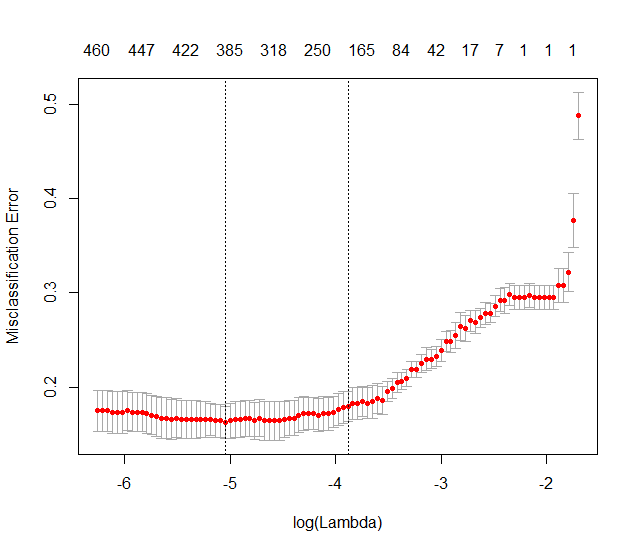
\includegraphics[width=0.8\linewidth]{lambda.png}
\end{figure}

To show you how little difference there is between the performance of the models using $\lambda$ = lambda.1se and $\lambda$ = lambda.min, see Table \ref{table:lambda}. For the performance in terms of accuracy etc, I would like to refer you to Table \ref{table:performanceOverview}.

\begin{table}[H]
\centering
\caption{Performance of Regularized Logistic Regression models, with a different value for $\lambda$.}
\label{table:lambda}
\begin{tabular}{|l|l|l|l|l|l|}
\hline
  & value of $\lambda$ & Accuracy & Precision & Recall  & F1-score \\
  \hline
1 & lambda.1se         & 76.88\%  & 78.67\%   & 73.75\% & 76.13\%  \\
2 & lambda.min         & 76.88\%  & 77.92\%   & 75\%    & 76.43\%  \\
\hline
\end{tabular}
\end{table}
\subsubsection{Classification Trees}
Building up a classification tree from the trainset is the third method we used for labeling reviews. First, we created a tree using parameters \textit{minbucket=2} and \textit{minsplit=5}. Speaking in terms of a classification tree, this means that a leaf node must at least contain 2 reviews and a node can only be splitted if it contains at least 5 reviews. Constructing this tree is basically done by splitting the set of reviews, based on the number of occurrences of a term in a review. Eventually, you stop splitting when there is no node left which satisfies the \textit{minsplit} constraint.

A problem which arises here is that the resulting classification tree becomes quite large and \textit{overfits} the training data. A better approach is to apply pruning, which is already mentioned in Section \ref{section:classTreesExplained}. 

The important hyper parameter in this case is the so called \textit{cost-complexity} pruning parameter (\textit{cp} in short). This parameter determines how much space for errors is tolerated when it comes down to splits in the tree. A higher value for \textit{cp} means a stricter policy and results in a smaller tree, whereas a lower value leads to less pruning (i.e. a larger tree). Thus, choosing a good value for \textit{cp} is important for obtaining a decent pruned tree from the original version.\\

\begin{table}[H]
\centering
\caption{Cost-complexity table of pruning the original tree.}
\label{table:cp}
\begin{tabular}{|l|l|l|l|l|l|}
\hline
   & CP          & nsplit & rel error & xerror   & xstd       \\
   \hline
1  & 0.409375000 & 0      & 1.000000  & 1.056250 & 0.03946589 \\
2  & 0.034375000 & 1      & 0.590625  & 0.590625 & 0.03606444 \\
3  & 0.031250000 & 2      & 0.556250  & 0.621875 & 0.03659366 \\
4  & \textbf{0.015625000} & \textbf{3}      & 0.525000  & \textbf{0.584375} & 0.03595257 \\
5  & 0.013541667 & 4      & 0.509375  & 0.593750 & 0.03611961 \\
6  & 0.012500000 & 10     & 0.409375  & 0.600000 & 0.03622844 \\
7  & 0.009375000 & 12     & 0.384375  & 0.618750 & 0.03654296 \\
8  & 0.006770833 & 23     & 0.278125  & 0.659375 & 0.03716464 \\
9  & 0.006250000 & 29     & 0.237500  & 0.681250 & 0.03746662 \\
10 & 0.004687500 & 47     & 0.125000  & 0.687500 & 0.03754880 \\
11 & 0.003125000 & 53     & 0.096875  & 0.696875 & 0.03766869 \\
12 & 0.000000000 & 58     & 0.081250  & 0.709375 & 0.03782230 \\
\hline
\end{tabular}
\end{table}

Based on Table \ref{table:cp}, we chose \textit{cp} = 0.015625, because this value leads to the lowest cross-validation error. The resulting classification tree is shown in Figure \ref{figure:classTree}. Although this tree is very simple, it performs pretty good. The exact performance measures of this classification are included in Table \ref{table:performanceOverview}.

\begin{figure}[H]
\label{figure:classTree}
\centering
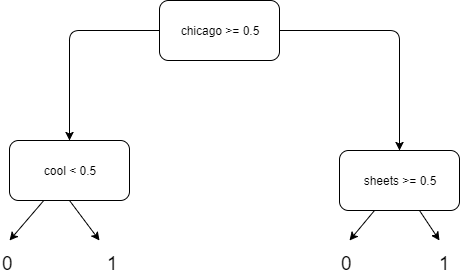
\includegraphics[width=0.7\linewidth]{classTree.png}
\end{figure}

Table \ref{table:treeResults} shows the differences in performance between the original tree and the pruned tree, shown in Figure \ref{figure:classTree}. Even though the pruned tree is much simpler, is outperforms the original, much more complicated tree.

\begin{table}[H]
\centering
\caption{Table containing the performance of a full-grown classification tree and a pruned tree, using $cp=0.015625$.}
\label{table:treeResults}
\begin{tabular}{|l|l|l|l|l|l|}
\hline
                         & \#of splits & Accuracy & Precision & Recall  & F1-score \\
                         \hline
Complete tree             & 58 & 61.88\%  & 62.67\%   & 58.75\% & 60.64\%  \\
Pruned tree (cp=0.015625) & 3  & 76.88\%  & 78.67\%   & 73.75\% & 76.13\%  \\
\hline
\end{tabular}
\end{table}


\subsubsection{Random Forests}
At last, we use the random forests algorithm for our classification problem. Building multiple trees and combining their resulting labels is another way to determine the label of a review. The performance of this method is dependent on the number of trees used, like you can see in Table \ref{table:forests}. Note that a higher number of trees improves the overall performance in general. Still, simply choosing a very high number does not always improve the classification. For instance, when you look at the case $n=100$ and compare it with the cases with a smaller number of trees, you can see that $n=100$ does not improve the performance. However, the model with 250 trees outperforms the other when it comes down to accuracy, presicion and the F1-score. So it seems that there the performance does not improve in certain ranges. Still, from Table \ref{table:forests} we conclude that having $n=250$ leads to the best classification.
\begin{table}[H]
\centering
\caption{Performance measures when applying random forests, where the number of trees is adjusted.}
\label{table:forests}
\begin{tabular}{|l|l|l|l|l|}
\hline
\# of trees & Accuracy & Precision & Recall  & F1-score \\
\hline
n=1             & 57.5\%   & 55.56\%   & 75\%    & 63.82\%  \\
n=10            & 65.63\%  & 64.04\%   & 71.25\% & 67.46\%  \\
n=25			& 75\%	   & 73.26\%   & 78.75\% & 75.91\%  \\
n=50            & 73.13\%  & 70.33\%   & \textbf{80\%}    & 74.85\%  \\
n=100           & 73.13\%  & 76.81\%   & 66.25\% & 71.14\%  \\
n=250           & \textbf{80.63\%}  & \textbf{85.51\%}   & 73.75\% & \textbf{79.20\%}  \\
\hline
\end{tabular}
\end{table}

\subsection{Bigrams}
Besides the experiments described above, we went a little further. Recall that these experiments only used unigrams. In other words, the features used represented single words. But besides looking at a single word as a feature, you can also use multiple words as a feature. Such features might improve understanding the context of a review in our case. So we also ran experiments with bigrams included in the feature set; features which represent two consecutive words in a document. Since we found over 40,000 bigrams, we removed the 2\% sparse terms to obtain a reasonable number of features. For Naive Bayes, we applied all pre-processing steps discussed in Section \ref{section:pre_processing}, whereas the other three algorithms only used the first three steps, described in Table \ref{table:pre-processing}.\\


\begin{table}[H]
\centering
\caption{Overview of the performance of the four algorithms discussed, based on whether or not they include bigrams in the feature set.}
\label{table:performanceOverview}
\begin{tabular}{|l|l|l|l|l|l|}
\Xhline{2\arrayrulewidth}
Classification method & Including bigrams & Accuracy & Precision & Recall  & F1-score \\
\Xhline{2\arrayrulewidth}
Naive bayes           & No                & 81.88\%  & 84\%      & 78.75\% & 81.29\%  \\
Naive bayes           & Yes               & 51.25\%  & 50.75\%   & 85\%    & 63.55\%  \\
\Xhline{2\arrayrulewidth}
Logistic Regression   & No                & 76.88\%  & 78.67\%   & 73.75\% & 76.13\%  \\
Logistic Regression   & Yes               & 72.5\%   & 80\%      & 60\%    & 68.57\%  \\
\Xhline{2\arrayrulewidth}
Classification tree   & No                & 64.38\%  & 64.56\%   & 63.75\% & 64.15\%  \\
Classification tree   & Yes               & 64.44\%  & 64.56\%   & 63.75\% & 64.15\%  \\
\Xhline{2\arrayrulewidth}
Random forests         & No                & 80.63\%  & 85.51\%   & 73.75\% & 79.20\%  \\
Random forests         & Yes               & 69.38\%  & 96.97\%   & 40\%    & 56.64\%  \\
\Xhline{2\arrayrulewidth}
\end{tabular}
\end{table}

\section{Discussion}

\subsection{Generative linear model versus Discriminative linear model}
% 1. How does the performance of the generative linear model (naive Bayes) compare to the discriminative linear model (logistic regression)?
In case of unigrams, comparing Naive Bayes to Regularized Logistic Regression, we observe that Naive Bayes performs better in accuracy, precision, recall and F1-score from Table \ref{table:performanceOverview}. To check if the difference in accuracy is significant we use the method described in Section \ref{section:evaluation}. 
\begin{table}[H]
\centering
\caption{Unigrams: The number cases in which Naive Bayes and Logistic regression agree and disagree.}
\label{table:NBLogUni}
\begin{tabular}{|l|l|l|}
\hline
\shortstack{Log. regression $\rightarrow$ \\ Naive Bayes $\downarrow$} & incorrect & correct \\
\hline
incorrect   & 13   & 16    \\
correct & 26   & 105     \\
\hline
\end{tabular}
\end{table}
The resulting $p$-value is $P(X \leq 16) + P(X \geq 26) = 0.16$, where $X \sim \texttt{Binom}(\pi = 0.5, n = 42)$. The found $p$-value is higher than 0.05 so the difference is so the difference in accuracy is not regarded as significantly different. For bigrams we perform the same type of significance testing as before. Here we observe that Regularized Logistic Regression has the better accuracy. The resulting $p$-value is $P(X \leq 17) + P(X \geq 32) = 0.04$, where $X \sim \texttt{Binom}(\pi = 0.5, n = 49)$. The found $p$-value is lower than 0.05, so the difference is so the difference in accuracy is regarded significantly different. 

Looking at precision, we observe that in case of unigrams Naive Bayes outperforms Regularized Logistic Regression but not by much. When using bigrams, we observe the same effect as with the accuracy: Regularized Logistic Regression outperforms Naive Bayes by quite a margin. We do not observe this effect when looking at the recall. The values F1-scores for both are similar in the case of unigrams and bigrams. 

The observation here is that in case of unigrams Naive Bayes performs better than Regularized Logistic Regression but the difference is not regarded as significant. The test set is not very large so we would have been able to make a better analysis if the test set was larger. In case of bigrams, Regularized Logistic Regression is the winner, this comes as no surprise looking at the large differences in accuracy Table \ref{table:performanceOverview}.

\subsection{Flexible classifiers versus Linear classifiers}
% 2. Is the random forests able to improve on the performance of the linear classifiers?
Regarding unigrams, the best performing linear classifier is Naive Bayes and the best performing flexible classifier is the random forest in terms of accuracy. To check if the difference in accuracy is significant we use the method described in Section \ref{section:evaluation}. 
\begin{table}[H]
\centering
\caption{Unigrams: The number cases in which Random forest and Naive Bayes agree and disagree.}
\label{table:flexLinUni}
\begin{tabular}{|l|l|l|}
\hline
\shortstack{Random forest $\rightarrow$ \\ Naive Bayes $\downarrow$} & incorrect & correct \\
\hline
incorrect   & 15   &  14   \\
correct & 15   &   116   \\
\hline
\end{tabular}
\end{table}
The resulting $p$-value is $P(X \leq  14) + P(X \geq 15) = 1.0$, where $X \sim \texttt{Binom}(\pi = 0.5, n =29)$. The found $p$-value is larger than 0.05 so the difference is not regarded as significant in terms of accuracy.
For bigrams we perform the same type of significance testing as before. The resulting $p$-value is $P(X \leq  19) + P(X \geq 45) = 0.001$, where $X \sim \texttt{Binom}(\pi = 0.5, n =64)$. The found $p$-value is smaller than 0.05 so the difference is regarded as significant in terms of accuracy. 

The observation here is that in case of unigrams the performance of both is similar in terms of all measures. For bigrams however, Random Forests outperform Naive Bayes in terms of accuracy but the recall drops by a lot. This means that in case of bigram usage, Random Forest have classify many more reviews as honest while they are actually fake. This effect is noticeable for the the precision of Naive Bayes when using bigrams, it classifies more honest reviews as fake when using bigrams. In the case of hotel reviews, it is much worse to classify an honest review as being fake because you discredit the review of an actual person that has put hard work in creating the review, this might result in lots of negative publicity.  

\subsection{Unigram features versus Bigrams}
% 3. Does performance improve by including bigram features, instead of using just unigrams?
Looking at Table \ref{table:performanceOverview}, we clearly see a trend of lower accuracies on all classifiers except for Classification trees. In case of classification trees the performance does not seem to improve or worsen. This result comes at quite a surprise because one would actually expect an increase in performance when one would use sequence information. One could speculate that bigrams actually give a skewed image of the reviews by suggesting that bigrams capture the context quite well. Trigrams would have been nice to test but fell outside the scope of the experiments. The least complex input data is the winner this time around. 

\subsection{Indications for fake and honest reviews}
So what are good indications for fake and honest reviews? Which features helped our classifiers the most? For Naive Bayes we have to look at the estimates word probabilities $\hat{P}(x|c)$ for both fake and honest reviews. For Regularized Logistic Regression we look at $p_i$ for fake reviews and $1-p_i$ for honest reviews which assigns a weight to every term based. For both these we will take the top 5 values based on their the terms which give the highest probability estimates given the class. For classification trees we looked at the first few splits to determine the top 5 for both cases. \\
The top-5 most important features are described per algorithm in Tables \ref{table:topFake} and \ref{table:topHonest}. 

\begin{table}[H]
\centering
\caption{The five most important terms (features) pointing towards a fake review.}
\label{table:topFake}
\begin{tabular}{|l|l|l|l|}
\hline
Rank & Naive Bayes & Reg. Logistic Regression & Trees \\
\hline
1 & Room      &  Grease  & Sheets\\
2 & Hotel     &  Star  & Looked \\
3 & Stay      &  Queens  & Mine \\
4 & One       &  Budapest  & Found\\
5 & Service   &  Tons  & Eggs \\
\hline
\end{tabular}
\end{table}

\begin{table}[H]
\centering
\caption{The five most important terms (features) pointing towards an honest review.}
\label{table:topHonest}
\begin{tabular}{|l|l|l|l|}
\hline
Rank & Naive Bayes & Reg. Logistic Regression & Trees \\
\hline
1 & Room    &  Chicago &  Chicago \\ 
2 & Hotel   &  Luxury  &  Cool \\
3 & Chicago &  Proved  &  Are\\
4 & Stay    &  Smell  &  Was\\
5 & Service &  Smelled  &  Windows\\
\hline
\end{tabular}
\end{table}

Looking at Table \ref{table:topFake}, we see that none of the three methods have an agreement on the top 5 terms for fake reviews. The same holds for the honest reviews (Table \ref{table:topHonest}), except for the term `Chicago'. Note that we did not actually look at the difference between the likelyhood of a feature leading to label 0 or 1. When you include this difference, than you may obtain features which discriminate fake and honest reviews the best.

\section{Conclusion}
You have read about four classification algorithms, which we applied in the context of classifying the truthfulness of hotel reviews. In terms of Naive Bayes, the pre-processing phase is very important. The runtime of Naive Bayes is strongly influenced by the number of features, thus filtering out as many irrelevant features as possible is critical if you want to retrieve results fast. Although Naive Bayes is the simplest model of all models we have seen, its performance is very impressive in comparison with the other algorithms (when only unigrams are used as features). However, Naive Bayes does not seem to cope well when we include bigrams, as is shown in Table \ref{table:performanceOverview}.

Logistic Regression is the second linear model and performed worse than Naive Bayes when only using unigrams. We have shown that not choosing a simpler model ($\lambda=$lambda.1se) performs as good as a more complicated model ($\lambda=$lambda.min) which minimized the cross-validation error. Unfortunately, adding bigrams also did not help with classification in this algorithm.

Using a classification tree was the third method we studied. When it comes down to pruning, choosing a value for the cost-complexity parameter is important. We have shown that, although the resulting pruned tree is very simple, it led to a better classification of the test set. Adding bigrams did not seem to change the performance.

The fourth and last method applied the concept of random forests. The number of trees chosen of this method has a big influence on the resulting classification, as shown in Table \ref{table:forests}. Although in our case  the case with the highest number of trees outperformed the others, this does not mean that you should always pick a very high number of trees.

So can these classification methods be used to detect fake reviews? In the case of unigrams the performance of Naive Bayes and Random forests is quite good terms of accuracy. Looking at the other measures, a higher precision is more important than high recall rate. It is more important to not classify honest reviews as fake than fake reviews being honest because this will discredit the user's review and might result in that users are less prone the write reviews. For both these two methods the precision and recall do not differ much. Since Naive Bayes is the simpler model, we recommend to use this in case of unigrams. Bigrams however, did not have the desired effect. This is something that can be investigated further in future works. Furthermore, other the performance of other larger k-grams is something to look at. What we noticed with bigrams is that, the accuracy dropped but the precision or recall increased in almost all cases. The increase in precision is particularly interesting to look at because of the reason stated above. The results obtained are interesting because the simple model came out as the winner in this case and we also obtained interesting result that can be investigated further in future works.


\bibliographystyle{unsrt}
\bibliography{sources}

\end{document}